\chapter{System Design}

This chapter presents the architecture of the simulation engine, organized around the principle that each component addresses a specific, identified problem. All deterministic logic---scoring functions, feature extraction, state management---is presented in pseudocode following the principle that non-LLM-wrapper logic must be fully transparent and reproducible.


\section{Architecture Overview}

The simulation engine processes a structured JSON simulation script through a phase-based dialogue loop. Each simulation script defines the scenario context, stakeholder roster (with OCEAN personality priors, incentives, and concerns), phase structure, and world events. Fig.~\ref{fig:architecture} illustrates the processing pipeline.

\begin{figure}[t]
    \centering
    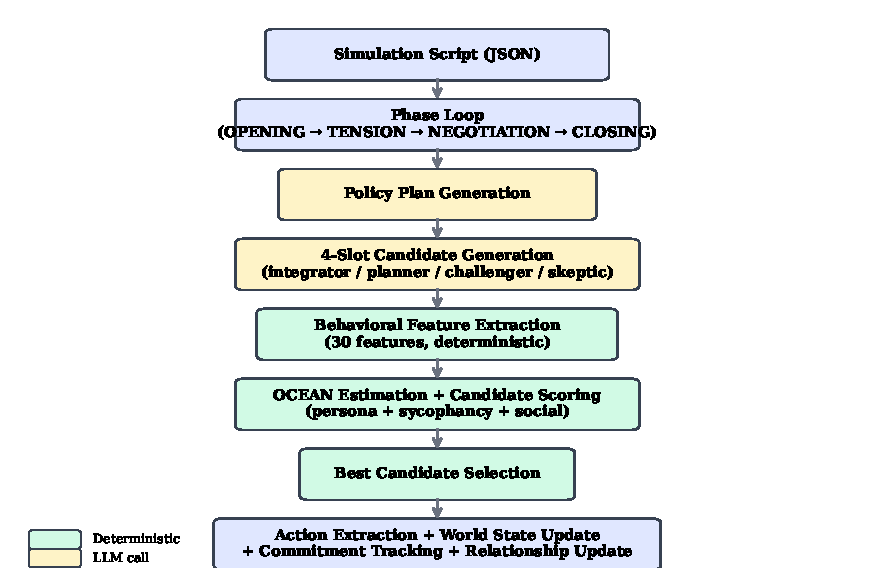
\includegraphics[width=\textwidth]{figures/fig1_architecture.pdf}
    \caption{System architecture pipeline. Yellow boxes indicate LLM calls; green boxes indicate deterministic (non-LLM) processing.}
    \label{fig:architecture}
\end{figure}

The engine operates in two modes: \textbf{guided} (outcome-anchored, where phase outcomes are specified in the script) and \textbf{exploratory} (open-ended, where outcomes emerge from agent interaction). Both modes share the same persona fidelity infrastructure.

\textbf{Technology stack:} Python, LangGraph (state machine orchestration), DeepSeek~V3 (text generation), sentence-transformers (semantic embeddings for convergence measurement).

Fig.~\ref{fig:layers} presents a cross-sectional view of the same architecture, organized by processing layer. Each layer operates on different data and at different abstraction levels: the Orchestration Layer manages phase sequencing and turn scheduling; the Generation Layer makes LLM calls for policy plans and candidate responses; the Control Layer applies deterministic scoring and selection; the State Layer maintains persistent memory (commitments, relationships, trait estimates); and the Action Layer extracts and applies structured world-state changes.

\begin{figure}[t]
    \centering
    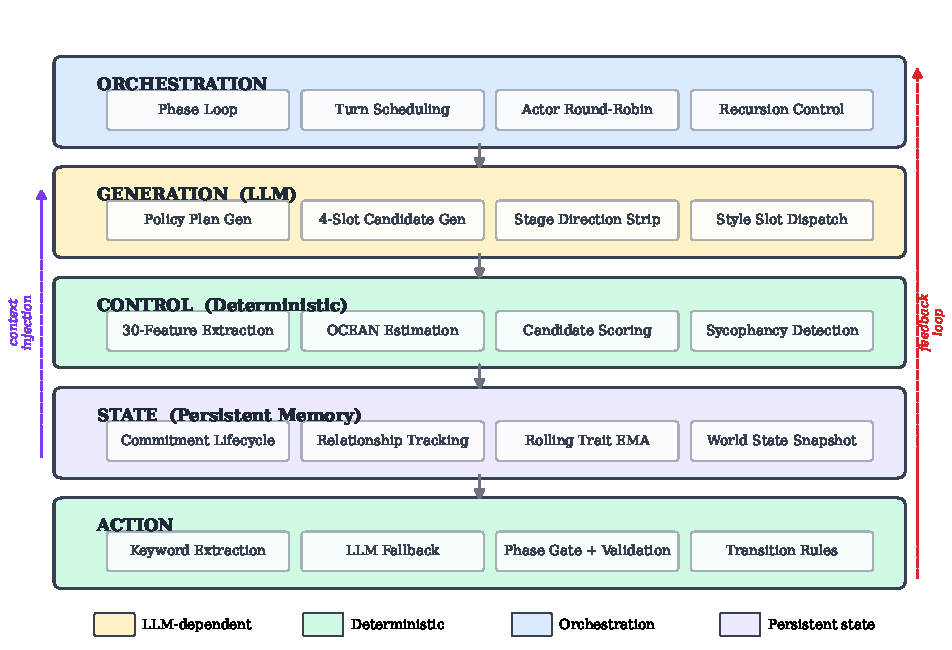
\includegraphics[width=\textwidth]{figures/fig8_layer_architecture.pdf}
    \caption{Cross-sectional layer architecture. Arrows indicate data flow between layers. Yellow shading indicates LLM-dependent processing; green indicates deterministic logic.}
    \label{fig:layers}
\end{figure}

Algorithm~\ref{alg:main_loop} presents the main simulation loop that orchestrates all components. Each turn generates four stylistically distinct candidates, scores them deterministically, and updates the persistent state ledger with commitments, relationships, and action proposals.

\begin{algorithm}[t]
\caption{Main Simulation Loop}
\label{alg:main_loop}
\begin{algorithmic}[1]
\Require simulation script $S$, condition $C$
\State $L \gets \textsc{InitLedger}(S)$ \Comment{State ledger}
\For{each phase $p \in S.\text{phases}$}
    \State $L.\textsc{ResolvePhaseCommitments}(p_{\text{prev}})$
    \For{each turn slot in $p$}
        \State $a \gets \textsc{ScheduleActor}(p, L)$
        \State $\text{ctx} \gets L.\textsc{SnapshotContext}(a)$
        \State $\pi \gets \textsc{GeneratePolicyPlan}(a, \text{ctx}, p)$ \Comment{LLM}
        \State $\mathcal{C} \gets \emptyset$
        \For{$s \in \{\text{integrator, planner, challenger, skeptic}\}$}
            \State $c \gets \textsc{Generate}(a, \text{ctx}, s)$ \Comment{LLM}
            \State $c.\text{score} \gets \textsc{Score}(c, a.\pi, p, L)$ \Comment{Alg~\ref{alg:scoring}}
            \State $\mathcal{C} \gets \mathcal{C} \cup \{c\}$
        \EndFor
        \State $c^* \gets \arg\max_{c \in \mathcal{C}} c.\text{score}$
        \State $L.\textsc{AppendTurn}(a, c^*.\text{text}, p)$
        \State $L.\textsc{UpdateCommitments}(a, c^*)$ \Comment{Alg~\ref{alg:commitment}}
        \State $L.\textsc{UpdateRelationships}(a, c^*.\text{text})$
        \State $\text{act} \gets \textsc{ExtractAction}(c^*, \pi, a, p)$ \Comment{Alg~\ref{alg:action}}
        \If{$\text{act} \neq \emptyset \land p \neq \text{OPENING}$}
            \State $L.\textsc{AppendProposal}(\text{act})$
        \EndIf
    \EndFor
    \State $\textsc{ArbitrateActions}(L.\text{proposals}(p))$
    \State $\textsc{ApplyTransitionRules}(S, L)$
\EndFor
\State \Return $L.\textsc{Result}()$
\end{algorithmic}
\end{algorithm}


\section{Persona State Controller}

\textbf{Problem:} LLMs exhibit persona drift in extended multi-turn conversations, gradually deviating from assigned personality profiles.

\textbf{Design Decision:} Rather than relying on LLM self-correction (which is unreliable) or post-hoc filtering (which wastes generation), the controller monitors behavioral fidelity at every turn and selects the most persona-consistent candidate from a pool of alternatives.

\textbf{Implementation:} At each turn, the controller extracts 30 behavioral features from the candidate's text, estimates the candidate's current OCEAN trait expression, compares it against the assigned personality prior, and applies a penalty proportional to the deviation.

\begin{algorithm}[t]
\caption{Candidate Scoring Function}
\label{alg:scoring}
\begin{algorithmic}[1]
\Require candidate text $c$, actor prior $\pi$, phase $p$, history $H$
\State $\mathbf{f} \gets \textsc{ExtractFeatures}(c)$ \Comment{30 features}
\State $\hat{\theta} \gets \textsc{EstimateOCEAN}(\mathbf{f}, H)$
\State $\text{drift} \gets \frac{1}{5}\sum_{t \in \text{OCEAN}} |\hat{\theta}_t - \pi_t|$
\State $\text{persona} \gets 1.0 - \text{drift}$
\State $\text{syc} \gets \textsc{DetectSycophancy}(\mathbf{f}, \pi, p)$
\State $\text{social} \gets \textsc{SocialAlignment}(\hat{\theta}, \pi)$
\State $\text{env} \gets \sum_{t} (\max(0, |\hat{\theta}_t - \pi_t| - \tau))^2$
\State $\mathbf{w} \gets \textsc{PhaseWeights}[p]$
\State \Return $w_p \cdot \text{persona} + w_s \cdot (1-\text{syc}) + w_o \cdot \text{social} - w_e \cdot \text{env}$
\end{algorithmic}
\end{algorithm}

The phase-specific weight modifiers (Table~\ref{tab:phase_weights}) reflect the observation that different phases exhibit different failure modes: during TENSION, sycophancy risk is highest; during CLOSING, envelope violations are most likely as agents converge toward a ``summarize and agree'' pattern.

\begin{table}[t]
\centering
\caption{Phase Weight Modifiers for Candidate Scoring}
\label{tab:phase_weights}
\begin{tabular}{lcccc}
\toprule
Phase & Persona & Sycophancy & Social & Envelope \\
\midrule
OPENING     & 1.2$\times$ & 0.8$\times$ & 1.0$\times$ & 1.0$\times$ \\
TENSION     & 1.0$\times$ & 1.8$\times$ & 1.4$\times$ & 1.0$\times$ \\
NEGOTIATION & 1.0$\times$ & 1.0$\times$ & 1.0$\times$ & 1.3$\times$ \\
CLOSING     & 1.3$\times$ & 1.0$\times$ & 1.0$\times$ & 1.4$\times$ \\
\bottomrule
\end{tabular}
\end{table}


\section{Behavioral Feature Extraction and OCEAN Estimation}

The controller extracts 30 linguistic features from each candidate text, organized by their primary OCEAN trait association. Table~\ref{tab:features} presents a representative subset (one per trait plus sycophancy indicators); the complete 30-feature specification is provided in Appendix~\ref{app:features}.

\begin{table}[t]
\centering
\caption{Representative Behavioral Features (subset of~30)}
\label{tab:features}
\begin{tabular}{p{2.5cm}p{1.5cm}p{6cm}}
\toprule
Feature & Trait & Why This Feature \\
\midrule
\texttt{idea\_count}          & \textbf{O} & Novel proposals introduced \\
\texttt{planning\_count}      & \textbf{C} & ``plan'', ``schedule'', ``timeline'' \\
\texttt{avg\_words\_per\_turn} & \textbf{E} & Word count per turn \\
\texttt{disagreement\_count}  & Low \textbf{A} & ``disagree'', ``however'', ``but'' \\
\texttt{hedge\_count}         & \textbf{N} & ``maybe'', ``perhaps'', ``might'' \\
\texttt{acknowledgment\_count} & Syc. & ``great point'', ``agree'' \\
\bottomrule
\end{tabular}
\end{table}

\textbf{Dynamic Calibration.} A critical design decision is the use of dynamic calibration against the conversation baseline when multiple speakers are present. Absolute feature counts are uninformative without context---a \texttt{planning\_count} of~3 may indicate high Conscientiousness in a casual discussion but low Conscientiousness in a project management meeting.

\begin{algorithm}[t]
\caption{OCEAN Estimation with Dynamic Calibration}
\label{alg:ocean}
\begin{algorithmic}[1]
\Require features $\mathbf{f}$, conversation history $H$
\If{multiple speakers in $H$}
    \State $\mathbf{b} \gets \textsc{ConversationBaseline}(H)$
    \For{each trait $t \in \{O, C, E, A, N\}$}
        \State $\hat{\theta}_t \gets \text{clip}\big(0.50 + \lambda_t \cdot (\text{raw}_t(\mathbf{f}) - b_t), 0, 1\big)$
    \EndFor
\Else
    \State Use static formula with absolute feature counts
\EndIf
\State \Return $\hat{\theta} = \{\hat{\theta}_O, \hat{\theta}_C, \hat{\theta}_E, \hat{\theta}_A, \hat{\theta}_N\}$
\end{algorithmic}
\end{algorithm}

The calibration coefficients $\lambda_t$ are: $\lambda_O = 0.55$, $\lambda_C = 0.55$, $\lambda_E = 0.65$, $\lambda_A = 0.50$, $\lambda_N = 0.50$. The higher coefficient for Extraversion ($0.65$) reflects the stronger signal-to-noise ratio of verbal features (word count, question frequency) compared to more subtle trait markers.

\textbf{Rolling Trait Estimation:} The state ledger maintains a rolling estimate of each actor's trait expression using exponential smoothing ($\alpha = 0.6$ for current turn, $0.4$ for history), preventing single-turn anomalies from triggering excessive correction.


\section{4-Slot Candidate Pool}

\textbf{Problem:} A single LLM generation per turn produces limited diversity and may yield suboptimal responses that happen to be sycophantic or persona-inconsistent.

\textbf{Design Decision:} Generate four candidate responses per turn, each with a distinct rhetorical style, and select the best according to the persona fidelity scoring function (Algorithm~\ref{alg:scoring}).

The four style slots are:
\begin{itemize}[leftmargin=*, itemsep=1pt]
    \item \textbf{Integrator:} seeks common ground; preferred actions include \texttt{assign\_owner}, \texttt{commit\_resource}, \texttt{publish\_update}.
    \item \textbf{Planner:} proposes structured plans; preferred actions include \texttt{set\_deadline}, \texttt{narrow\_scope}, \texttt{pilot}.
    \item \textbf{Challenger:} questions assumptions; preferred actions include \texttt{preserve\_autonomy}, \texttt{request\_evidence}, \texttt{escalate}.
    \item \textbf{Skeptic:} expresses doubt; preferred actions include \texttt{audit\_compliance}, \texttt{defer\_decision}, \texttt{request\_evidence}.
\end{itemize}

\textbf{Cost-Diversity Tradeoff:} Each turn requires 4 LLM generation calls, resulting in approximately 88 API calls per simulation run (11 average turns $\times$ 4 slots $\times$ 2 actors per turn). A complete simulation takes approximately 3~minutes. This cost is justified by the diversity it provides: without multiple candidates, the controller has no alternatives from which to select persona-consistent responses.


\section{Sycophancy Detection}

\textbf{Problem:} RLHF-trained LLMs exhibit a systematic bias toward agreement, causing multi-agent simulations to converge rapidly on consensus.

\textbf{Design Decision:} A multi-layered detection system that penalizes sycophantic candidates during scoring, with sensitivity calibrated to the scenario's structural polarity and each actor's strategic disposition.

\begin{algorithm}[t]
\caption{Sycophancy Risk Detection}
\label{alg:sycophancy}
\begin{algorithmic}[1]
\Require features $\mathbf{f}$, actor prior $\pi$, phase $p$
\State \textit{// Layer 1: Keyword-based detection}
\State $r \gets f_{\text{ack}} \times 0.15 + f_{\text{excl}} \times 0.10$
\State \textit{// Layer 2: Structural polarity amplification}
\If{scenario polarity $> 0.7$}
    \State $r \gets r \times 1.3$ \Comment{High-conflict $\Rightarrow$ agreement suspicious}
\EndIf
\State \textit{// Layer 3: Strategic disposition adjustment}
\If{actor disposition $\in \{$adversarial, competitive$\}$}
    \State $r \gets r \times 1.5$
\EndIf
\State \textit{// Layer 4: Low Agreeableness adjustment}
\If{$\pi_A < 0.4$}
    \State $r \gets r \times 1.2$
\EndIf
\State \Return $\text{clip}(r, 0, 1)$
\end{algorithmic}
\end{algorithm}


\section{Commitment Lifecycle}

\textbf{Problem:} Agents make commitments (``I will prepare the draft by Friday'') but fail to follow through or contradict themselves in subsequent turns.

\textbf{Design Decision:} Track all commitments in a state ledger with lifecycle management: extraction $\to$ monitoring $\to$ fulfillment detection $\to$ staleness resolution.

A critical design insight emerged from early experiments: instructing agents to ``stay consistent'' (directive approach) caused diversity to collapse to 0.45 as agents rigidly maintained their initial positions. The successful approach is \textit{informational}: presenting ``Your prior positions: [list]'' without any instruction, allowing the LLM to decide how to use that information. This soft prompt injection achieves zero contradictions while maintaining behavioral diversity---a result consistent with the psychological principle that identity awareness promotes consistency more effectively than behavioral commands.

\begin{algorithm}[t]
\caption{Commitment Lifecycle Management}
\label{alg:commitment}
\begin{algorithmic}[1]
\Require actor $a$, text $t$, turn index $i$, phase $p$, max age $\tau = 8$
\State \textit{// Stage 1: Extract new commitments}
\State $\mathcal{K} \gets \textsc{ExtractCommitments}(t, i, p)$ \Comment{LLM}
\For{each $k \in \mathcal{K}$}
    \State $k.\text{status} \gets \text{``open''}$; \quad $L.\text{commitments}[a] \mathrel{+}= \{k\}$
\EndFor
\State \textit{// Stage 2: Fulfillment detection}
\For{each $k \in L.\textsc{OpenCommitments}(a)$}
    \If{$\textsc{CheckFulfilled}(t, k)$} \Comment{LLM}
        \State $k.\text{status} \gets \text{``fulfilled''}$
    \EndIf
\EndFor
\State \textit{// Stage 3: Phase-based resolution}
\For{each $k$ where $k.\text{due\_phase} = p$}
    \State $k.\text{status} \gets \text{``resolved''}$
\EndFor
\State \textit{// Stage 4: Staleness resolution}
\For{each $k \in L.\textsc{OpenCommitments}(a)$}
    \If{$i - k.\text{created\_at} > \tau$}
        \State $k.\text{status} \gets \text{``stale''}$
    \EndIf
\EndFor
\State \textit{// Soft prompt injection (informational, not directive)}
\State $\text{prior} \gets [k.\text{summary} \mid k \in L.\textsc{OpenCommitments}(a)]$
\State Inject ``Your prior positions: $\text{prior}$'' into generation prompt
\end{algorithmic}
\end{algorithm}


\section{Action Layer}

\textbf{Problem:} Dialogue text alone cannot capture the structural actions stakeholders take during deliberation (assigning tasks, requesting evidence, escalating to authority). Without action extraction, the simulation produces conversation but not traceable decision-making.

\textbf{Design Decision:} Define 12 structured action types organized in 7 families (Table~\ref{tab:actions}), with a hybrid extraction pipeline (deterministic keyword matching with LLM fallback) and phase-gated validation.

\begin{table}[t]
\centering
\caption{12 Structured Action Types}
\label{tab:actions}
\begin{tabular}{llc}
\toprule
Family & Action Type & State Delta \\
\midrule
Ownership   & \texttt{assign\_owner}      & trust +0.04 \\
Evidence    & \texttt{request\_evidence}   & uncertainty $-$0.04 \\
Comms       & \texttt{publish\_update}     & alignment +0.04 \\
\multirow{2}{*}{Scope}
            & \texttt{narrow\_scope}       & uncertainty $-$0.04 \\
            & \texttt{pilot}               & risk $-$0.08 \\
\multirow{2}{*}{Resourcing}
            & \texttt{commit\_resource}    & confidence +0.08 \\
            & \texttt{allocate\_budget}    & confidence +0.08 \\
\multirow{2}{*}{Timing}
            & \texttt{set\_deadline}       & uncertainty $-$0.04 \\
            & \texttt{defer\_decision}     & tension $-$0.04 \\
\multirow{3}{*}{Governance}
            & \texttt{preserve\_autonomy}  & tension +0.08 \\
            & \texttt{escalate}            & tension +0.12 \\
            & \texttt{audit\_compliance}   & uncertainty $-$0.08 \\
\bottomrule
\end{tabular}
\end{table}

The action extraction pipeline operates in four stages: (1)~detect action-bearing turns using keyword cues; (2)~extract action type via keyword matching (deterministic) with LLM fallback; (3)~apply phase gate (OPENING operates in shadow mode---actions are detected but not executed); (4)~validate and execute world-state delta updates. Algorithm~\ref{alg:action} formalizes this pipeline with its sparse gate mechanism.

\begin{algorithm}[t]
\caption{Action Extraction Pipeline}
\label{alg:action}
\begin{algorithmic}[1]
\Require text $t$, policy plan $\pi$, actor $a$, phase $p$, threshold $\sigma = 0.62$
\State \textit{// Stage 1: Policy-based action (highest priority)}
\If{$\pi.\text{planned\_action} \neq \emptyset$}
    \State $\alpha \gets \textsc{Normalize}(\pi.\text{planned\_action})$
    \If{$\textsc{ActivationScore}(\alpha) \geq \sigma$} \Comment{Sparse gate}
        \State $q \gets \textsc{Validate}(\textsc{Proposal}(\alpha, \text{src}{=}\text{``planned''}))$
        \If{$q.\text{status} = \text{``proposed''}$} \Return $q$ \EndIf
    \EndIf
\EndIf
\State \textit{// Stage 2: Heuristic keyword extraction}
\If{$\textsc{DetectActionBearing}(t)$}
    \State $\text{type} \gets \textsc{KeywordMatch}(t, \text{CUE\_PATTERNS})$
    \State $\text{key} \gets \textsc{KeywordMatch}(t, \text{STATE\_HINTS})$
    \State $\text{str} \gets \textsc{DetectStrength}(t)$ \Comment{high / medium / low}
    \State $\text{conf} \gets 0.45 \pm \Delta_{\text{modal}}$ \Comment{$\pm 0.18$ strong modals}
    \State $q \gets \textsc{Validate}(\textsc{Proposal}(\text{type}, \text{key}, \text{src}{=}\text{``heuristic''}))$
    \If{$q.\text{status} = \text{``proposed''} \land \textsc{ActivationScore}(q) \geq \sigma$}
        \State \Return $q$
    \EndIf
\EndIf
\State \textit{// Stage 3: LLM fallback (deterministic temperature)}
\If{$\textsc{DetectActionBearing}(t)$}
    \State $q \gets \textsc{LLMExtract}(t, \text{allowed\_types}, T{=}0)$ \Comment{LLM}
    \If{$\textsc{Validate}(q).\text{status} = \text{``proposed''}$} \Return $q$ \EndIf
\EndIf
\State \Return $\emptyset$
\end{algorithmic}
\end{algorithm}


\section{Strategic Disposition}

\textbf{Problem:} Without differentiated strategic orientations, all actors default to neutral-cooperative behavior, weakening the conflict dynamics essential to realistic deliberation.

\textbf{Design Decision:} Each actor is assigned a \texttt{strategic\_disposition} (\texttt{cooperative}, \texttt{neutral}, \texttt{competitive}, \texttt{adversarial}) with a \texttt{disposition\_strength} ($0.0$--$1.0$). This disposition operates at three levels: (1)~system prompt tone modification, (2)~action type bias in the policy plan, and (3)~sycophancy detection threshold adjustment (see Algorithm~\ref{alg:sycophancy}, Layer~3). The default disposition is \texttt{neutral}, ensuring backward compatibility with existing simulation scripts.
